\chapter{Introduction}
\section{Overview}
Information technology changes rapidly, at the same time the requirements of the information users also change. With the development of the technologies, it is possible to handle the huge amount of data in a short time. Information technology is the base for most of the companies. In the competitive market, the companies who have current information about the business and the competitors they are more stable in the market.  All decision making and strategy setting depend on current business information. It is very important to get the reliable, valuable and concrete information on right time. 
To achieve the real-time information, the main challenge rises between the operative system and the analytical system. Operative system store the current transactional data and need to response every sub-seconds for a business transaction. Due to the technical reason analytical system have to separate from the operative system. The reporting speed depends on how fast the data arrives from operative system to analytical system. To minimize this gap, some techniques has invented like In-memory database technique by SAP. It is giving nearly the real-time information.
However, the companies invest huge on Business Intelligence, lots of projects failed for wrong data processes. Besides the selection of good hardwires and software, it is also important to define the optimal data process to get the efficient results from the system. 
 




\cite{}
\section{Motivation}
Almost all companies, the information technology plays significant role in their daily work. From the process monitoring to decision making all are based on the current status of the company. By the help of the Information technology, now the  information is more accurate and current than before. In the big companies like BMW it is nearly fully automatize, nearly every process are captured and store into the database to get the most current status of the production and speed up the decision making process. Is that because, if the production is off for some hours then the company have to count huge amount of money. It is very important to make the system stable for all time. To maintain such kind of system is really challenging and at the same time it is also interesting to see how they are dealing with it.\\\\
In BMW, the existing data model is immense, complex and old but it is working. The existing system mainly consists of more than four hundred relational tables, more than ten thousand objects, lot of joins, business intelligence tools and several servers. The reports are generated in various time periods, different work shifts, and different department to assist the decision making and process development.There are several departments who are responsible for the reporting. Even though different plants and reporting departments are using a similar data model but the report processing methods are not the similar. Every plant using individual techniques to fetch the data from databases. Some techniques are working well, some takes more time  to generate a report.  In the case of the complex report, the plant report coordinator faces lot of problems. At this point, if,it is possible to make some core functions reusable, which can be used by all reporting departments then it can save lot of time and cost for the company.\\

Although the work flow and the data structure is complex and hard to understand in a short period of time, a little tuning of the data process will do a huge impact to the large number of users.\\ 


\section{Problem description }
Although, the system is running properly but the requirements of the information consumers (managers) were not fulfilled. After considering their requirements, it was noticed that some functions ware missing from the root system and  some necessary functions should include to fulfill the requirements. According to the company rules, there is some restriction which will not allow to  change something in the root system easily. \\

Figure 1.1 illustrate the basic data flow model of the current system. From the database the data coming to the SAP system. After adding some functions and semantic layer creation it send to the report development process. Here, some data is missing from the database. That's the reason it is not possible to build those functions. However, I have to find an alternative way which will solve the missing function problem without touching the main database design.\\
\begin{figure}[!ht]
	\centering
		%[natürliche Breite in Pixeln, natürliche Höhe in Pixeln, Abhängigkeit von der Textbreite]
		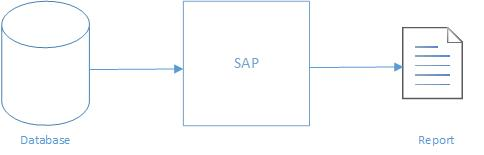
\includegraphics[width=pt, height=155pt, width=1.0\textwidth]{images/1.jpg}
	\caption{Basic model of the current system}
	\label{fig:1}
\end{figure}

In the current database, the available dates are only working days. Holidays are not storing in the database. Future dates and holidays are not possible to get from the database because those dates are not exist in the database table.  For the reason, some problems are occurring and some functions are not possible to develop to make the reporting process more flexible. \\

Figure 2 shows, the current status of the dates and what is expecting in future. In this figure, considering current date is 15.06.17. In the left side of the figure, it shows, the dates are available till current date and these dates are without the holiday. In the right side, it is showing the expecting date which will come with the future dates along with holiday dates.\\
\begin{figure}[!ht]
	\centering
		%[natürliche Breite in Pixeln, natürliche Höhe in Pixeln, Abhängigkeit von der Textbreite]
		
\includegraphics[width=pt, height=122pt, width=1.0\textwidth]{images/2.jpg}
	\caption{Existing dates and target dates}
	\label{fig:2}
\end{figure}

The main problems are mentioning below: 

\begin{itemize}
\item Dynamic data filtering/restriction functionalities for various time period.
\item To calculate the month cumulative, year cumulative, week cumulative are not possible because the future dates are not available in the database.
\item Clear representation of the production in the report.
\item The problem is to build some reusable functions. Different plants are using  different objects for the date functions. There is no common functions or common object for this.
\item The problem is to make a standard report template.
\item The Report performance is not satisfactory level.
\item It is hard to maintenance.
\item Another problem is related to KPIs. When a report changes to different time periods then KPIs are not generating correctly. Every time needs to changes the function for the new time period. For example, last day production, last month production, this week, last week, this year etc. When a report changes from current month to last month then KPIs are not generating correctly.
\end{itemize}

\section{Goals and Objectives}
The main goal of this Master thesis is to find out the new concepts for data optimization and report standardization which will convey the re-usability, scalability functions and accommodate with the end user requirements. To achieve this goal the main task will be:\\

\begin{itemize}
\item  Optimization of current data model and processes.
\item  Add dynamic functionalities which will help to speed up the report development.
\item  Understanding the information consumer's requirements
\item  Build a standard reporting template.
\end{itemize}

\section{Presentation of the Company}
\subsection{BMW Group}
In 1916, the Flugmaschinefabrik Gustav otto company had marged into Bayerische Flugzeug-Werke AG (BFG) at government behest. In 1917, the Rapp Motorenwerke company became Bayerische Motoren Werke GmbH. In 1918, Bayerische Motoren Werke GmbH converted into public limited company and after four years it transferred its engine construction operation including its company and brand name to BFG. The date of BFG's founding date is consider as Bayerische Motoren Werke AG (BMW) foundation date, 7 march 1916.\footnote{BMW AG, https://www.bmwgroup.com/en/company/history.html } \newline\\
With its three brands BMW, MINI and Rolls-Royce, the BMW Group is the world’s leading premium manufacturer of automobiles and motorcycles and also provides premium financial and mobility services. As a global company, the BMW Group operates 31 production and assembly facilities in 14 countries and has a global sales network in more than 140 countries.\footnote{BMW AG, https://www.bmwgroup.com/en/company/business-segments.html, 2016} According to Figure 1.3, there are 124,729 employees working worldwide. In the automotive segment 90.5 percent, in the motorcycle segment 2.7 percent and in the financial segment 6.7 percent employees are working. In 2016, 2,367,603 automobiles sold and the total revenue was 94,163,000,000 euros.

\begin{figure}[!ht] 
	\centering
		%[natürliche Breite in Pixeln, natürliche Höhe in Pixeln, Abhängigkeit von der Textbreite]
		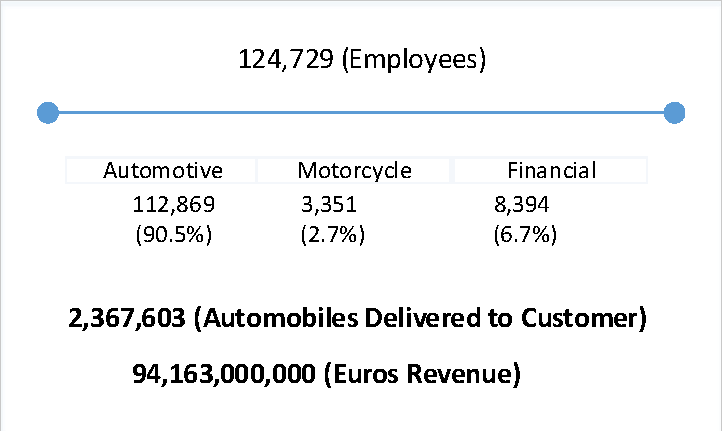
\includegraphics[width=414pt, height=238pt, width=1.0\textwidth]{images/BMW1.pdf}
	\caption[BMW Group Key Figure 2016]{BMW Group Key Figure 2016\footnotemark}
	\label{fig:BMW1}
\end{figure}
\footnotetext{BMW AG, https://www.bmwgroup.com/en/company.html, 2016 )}\newpage

\subsection{Plant Dingolfing}
BMW Group Plant Dingolfing is the BMW Group's biggest vehicle production site in Europe. In every day this plant producing about 1,600 cars and annually about 340,000 cars. Currently this plant producing 3, 4, 5, 6 and 7 Series, and also segments for BMW's electric vehicles and auto bodies for Rolls-Royce Motor Cars. Over that, Dingolfing is at the focal point of the BMW Group's worldwide extra parts logistics network. Altogether, the area has a workforce of more than 17,500 individuals, in addition to 800 students. This plant situated in Lower Bavaria.\newline 

BMW Group plant Dingolfing is 50 years old and more than nine million BMW vehicles have been produce at the plant. There are four main departments in Dingolfing plant. They are press shop, body shop, assembly and paint. In the press shop, more than 40 press system produce about 2,500 different parts from fuel tank caps to side frames, with the sheet thickness ranging from 0.65 to 3 mm. In the body shop, most of the work done by about 2,000 industrial robots. In the paint shop, paint the body of the cars. Paint shop offer more than 300 series and special colors. In the assembly, more than 6,0000 workers assemble the painted car bodies with the equipments selected by the customers. \footnote{BMW AG, http://www.bmwgroup-plants.com/en/dingolfing.html, 2017}
\begin{figure}[!ht] 
	\centering
		%[natürliche Breite in Pixeln, natürliche Höhe in Pixeln, Abhängigkeit von der Textbreite]
		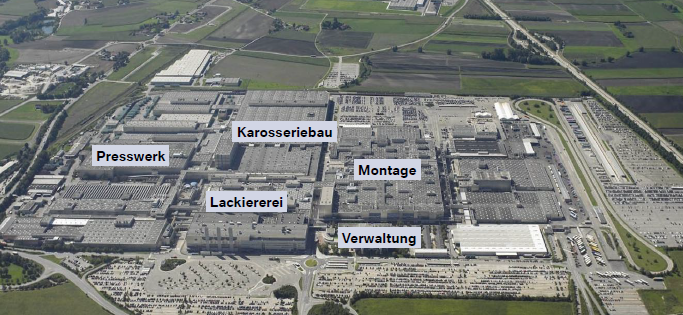
\includegraphics[width=414pt, height=238pt, width=1.0\textwidth]{images/BMW2.PNG}
	\caption[Plant Dingolfing, Work 2.40]{Plant Dingolfing, Work 2.40\footnotemark}
	\label{fig:BMW2}
   \end{figure}
    \footnotetext{(BMW AG, BMW Work Presentation 2015, 2016) https://www.bmwgroup.com/en/company.html)}

\subsection{Quality Management Department, Paint Shop}

Quality management department  responsible for quality, work safety and environmental management, quality control, Q-info management and the proper execution of the sectoral audit of the painted body. The area of responsibility covers the entire process chain, starting with the technology of forming, the technology of bodywork construction and the technology surface.\footnote{(BMW AG,TD-300 - Quality Management, 2016)}\\

TD-300, Q-info management is a part of quality management department. The main task is to generate quality reports over the entire paint shop. In the paint shop there are many small  processes for car painting. Every process instantly capture by the different capturing system. All the captured data store in the database. Those data are use for reporting. This department are serves various types of reports for different level of management.\newpage   
\section{Thesis outline}
The rest of this report is divided into five chapters - Data modeling techniques, Analysis, Optimization process, Report standardization , Proof of concept and conclusion.\\

The data modeling  chapter begins with the common approaches of data modeling techniques. Furthermore, the benefit of dimensional modeling  and few core concept about facts and dimensional table and E/R data model. \\

The analysis chapter describes the current reporting process. It is contains the existing data model, tools and the report development process of the current system.\\

In the optimization  chapter, showing about the optimization process of current system by using SAP BO tools and comparison between the current process and newly optimize process of the system.\\

In report standardization chapter, the inputs for the standard report and standard reporting template are discussed.\\

In the proof of concept chapter, the performance of the current solution for both the optimize data model and the standard report template are presented.This is divided into a set of test cases with the actual usage scenarios.\\

The report is ended up with the conclusion chapter. 